\section{Supplementary Material: Forman Profile}
\label{sec:forman_supplementary}

This section collects the per-dataset heatmap figures referenced in Section~\ref{sec:forman_profile}, together with the global summary tables for the analyses not shown in the main text: the other-Laplacian ablation, the cross-comparison, and the normalised Joint diffusion regime.

\subsection{Per-dataset examples}

\begin{figure}[H]
    \centering
    
\includegraphics[width=\linewidth]{../Deck_slides/heatmaps/GeneralSheaf/normalised_true/roman_empire_GeneralSheaf_d5_5L_Norm_True_heatmap.pdf}
    \caption{From left to right, starting from the top: Spearman correlation, Pearson correlation, Wasserstain distance, RMSE and NMRSE between the normalized Sheaf Laplacian and the topological reference. Here we consider a node classification task performed on the Roman Empire dataset. Relevant hyperparameters are stalk dimension = $5$ and number of layers = $5$. }
    \label{fig: RM_Norm}
\end{figure}

\begin{figure}[H]
    \centering
    
\includegraphics[width=\linewidth]{../Deck_slides/heatmaps/GeneralSheaf/normalised_false/citeseer_GeneralSheaf_d5_4L_Norm_False_heatmap.pdf}
    \caption{From left to right, starting from the top: Wasserstein distance against the topological reference, Wasserstein distance against the zero reference, Pearson correlation and NRMSE against  the topological reference, and RMSE against the zero reference. Here we consider a node classification task performed on the Citeseer dataset. Relevant hyperparameters are stalk dimension = $5$ and number of layers = $4$.}
    \label{fig: Citeseer_Not_Norm}
\end{figure}

\begin{figure}[H]
    \centering
    
\includegraphics[width=\linewidth]{../Deck_slides/heatmaps/GeneralSheaf/normalised_true_other/pubmed_GeneralSheaf_d5_4L_Norm_False_heatmap.pdf}
    \caption{From left to right, starting from the top: Spearman correlation, Pearson correlation, Wasserstein distance, RMSE and NRMSE between the \emph{other Laplacian} and the topological reference. Here the restriction maps are learnt with \texttt{norm=False}, and the normalised Laplacian $\widetilde{\Delta}_{\mathcal{F}}$ built from those same maps is the one evaluated: the content is therefore normalised, while the training regime is not. Here we consider a node classification task performed on the Pubmed dataset. Relevant hyperparameters are stalk dimension = $5$ and number of layers = $4$. }
    \label{fig: Pubmed_Other_Norm}
\end{figure}

\begin{figure}[H]
    \centering
    
\includegraphics[width=\linewidth]{../Deck_slides/heatmaps/GeneralSheaf/normalised_false_other/pubmed_GeneralSheaf_d5_4L_Norm_True_heatmap.pdf}
    \caption{From left to right, starting from the top: Wasserstein distance against the topological reference, Wasserstein distance against the zero reference, Pearson correlation and NRMSE against the topological reference, and RMSE against the zero reference. Here the restriction maps are learnt with \texttt{norm=True}, and the unnormalised Laplacian $\Delta_{\mathcal{F}}$ built from those same maps is the one evaluated: the content is therefore unnormalised, while the training regime is not. Here we consider a node classification task performed on the Pubmed dataset. Relevant hyperparameters are stalk dimension = $5$ and number of layers = $4$. }
    \label{fig: Pubmed_Other_Unnorm}
\end{figure}

\begin{figure}[H]
    \centering
    
\includegraphics[width=\linewidth]{../Deck_slides/heatmaps/comparison/norm_true_vs_other_norm_false/pubmed_GeneralSheaf_d5_4L_norm_true_primary_vs_other_norm_false_heatmap.pdf}
    \caption{From left to right, starting from the top: Spearman correlation, Pearson correlation, Wasserstein distance, RMSE and NRMSE. This is the cross-comparison along the normalised column: both profiles come from the normalised Laplacian $\widetilde{\Delta}_{\mathcal{F}}$, one obtained from maps trained with \texttt{norm=True} and the other from maps trained with \texttt{norm=False}. The metrics are therefore computed between the two learnt profiles, and not against a reference. Here we consider a node classification task performed on the Pubmed dataset. Relevant hyperparameters are stalk dimension = $5$ and number of layers = $4$. }
    \label{fig: Pubmed_Cross_A}
\end{figure}

\begin{figure}[H]
    \centering
    
\includegraphics[width=\linewidth]{../Deck_slides/heatmaps/comparison/norm_false_vs_other_norm_true/pubmed_GeneralSheaf_d5_4L_norm_false_primary_vs_other_norm_true_heatmap.pdf}
    \caption{From left to right, starting from the top: Spearman correlation, Pearson correlation, Wasserstein distance, RMSE and NRMSE. This is the cross-comparison along the unnormalised column: both profiles come from the unnormalised Laplacian $\Delta_{\mathcal{F}}$, one obtained from maps trained with \texttt{norm=False} and the other from maps trained with \texttt{norm=True}. The metrics are therefore computed between the two learnt profiles, and not against a reference. Here we consider a node classification task performed on the Pubmed dataset. Relevant hyperparameters are stalk dimension = $5$ and number of layers = $4$. }
    \label{fig: Pubmed_Cross_B}
\end{figure}

\begin{figure}[H]
    \centering
    
\includegraphics[width=0.8\linewidth]{../Deck_slides/heatmaps/JointSheafParams/normalised_false/first_maps_identity/wisconsin_JointSheafParams_d2_2L_Norm_False_first_maps_identity_heatmap.pdf}
    \caption{From left to right, starting from the top: Wasserstein distance against the topological reference, Wasserstein distance against the zero reference, Pearson correlation and NRMSE against the topological reference, and RMSE against the zero reference, between the unnormalised joint-diffusion sheaf Laplacian and its references, starting from the identity sheaf $\mathcal{F}^{(0)} = I_d$. Here we consider a node classification task performed on the Wisconsin dataset. Relevant hyperparameters are stalk dimension = $2$ and number of layers = $2$. }
    \label{fig: Wisconsin_Joint_Unnorm}
\end{figure}

\begin{figure}[H]
    \centering
    
\includegraphics[width=\linewidth]{../Deck_slides/heatmaps/JointSheafParams/normalised_false/first_maps_identity/questions_JointSheafParams_d5_4L_Norm_False_first_maps_identity_heatmap.pdf}
    \caption{From left to right, starting from the top: Wasserstein distance against the topological reference, Wasserstein distance against the zero reference, Pearson correlation and NRMSE against the topological reference, and RMSE against the zero reference, between the unnormalised joint-diffusion sheaf Laplacian and its references, starting from the identity sheaf $\mathcal{F}^{(0)} = I_d$. Here we consider a node classification task performed on the Questions dataset. Relevant hyperparameters are stalk dimension = $5$ and number of layers = $4$. }
    \label{fig: Questions_Joint_Unnorm}
\end{figure}

\begin{figure}[H]
    \centering
    
\includegraphics[width=\linewidth]{../Deck_slides/heatmaps/JointSheafParams/normalised_true/first_maps_identity/minesweeper_JointSheafParams_d3_3L_Norm_True_first_maps_identity_heatmap.pdf}
    \caption{From left to right, starting from the top: Spearman correlation, Pearson correlation, Wasserstein distance, RMSE and NRMSE, between the normalised joint-diffusion sheaf Laplacian and the topological reference, starting from the identity sheaf $\mathcal{F}^{(0)} = I_d$. Here we consider a node classification task performed on the Minesweeper dataset. Relevant hyperparameters are stalk dimension = $3$ and number of layers = $3$, smaller than in the unnormalised regime due to the instability of normalised joint diffusion. }
    \label{fig: Minesweeper_Joint_Norm}
\end{figure}

\subsection{Global summary tables}

\begin{table}[H]
\centering
\definecolor{tabglobaljointnorm0}{rgb}{1.0,1.0,0.8}
\definecolor{tabglobaljointnorm1}{rgb}{0.9961,0.797,0.4046}
\definecolor{tabglobaljointnorm2}{rgb}{0.993,0.5825,0.2481}
\definecolor{tabglobaljointnorm3}{rgb}{0.9961,0.7778,0.3839}
\definecolor{tabglobaljointnorm4}{rgb}{0.9921,0.5491,0.2342}
\definecolor{tabglobaljointnorm5}{rgb}{0.9961,0.7346,0.3374}
\definecolor{tabglobaljointnorm6}{rgb}{0.991,0.4793,0.2143}
\definecolor{tabglobaljointnorm7}{rgb}{0.9944,0.6372,0.2717}
\definecolor{tabglobaljointnorm8}{rgb}{0.9832,0.2955,0.1619}
\definecolor{tabglobaljointnorm9}{rgb}{0.9928,0.578,0.2461}
\definecolor{tabglobaljointnorm10}{rgb}{0.8072,0.0452,0.1316}
\definecolor{tabglobaljointnorm11}{rgb}{0.9925,0.5643,0.2402}
\definecolor{tabglobaljointnorm12}{rgb}{0.502,0.0,0.149}
\definecolor{tabglobaljointnorm13}{rgb}{0.9906,0.4561,0.2076}
\definecolor{tabglobaljointnorm14}{rgb}{1.0,0.9801,0.7513}
\definecolor{tabglobaljointnorm15}{rgb}{1.0,0.9402,0.6538}
\definecolor{tabglobaljointnorm16}{rgb}{0.9984,0.8971,0.5596}
\definecolor{tabglobaljointnorm17}{rgb}{0.9961,0.8498,0.4615}
\definecolor{tabglobaljointnorm18}{rgb}{0.9961,0.7634,0.3684}
\definecolor{tabglobaljointnorm19}{rgb}{0.9955,0.6781,0.2894}
\definecolor{tabglobaljointnorm20}{rgb}{0.9933,0.5962,0.254}
\definecolor{tabglobaljointnorm21}{rgb}{0.9888,0.3398,0.1744}
\definecolor{tabglobaljointnorm22}{rgb}{0.9463,0.2187,0.1412}
\definecolor{tabglobaljointnorm23}{rgb}{0.8867,0.0996,0.1107}
\definecolor{tabglobaljointnorm24}{rgb}{0.8025,0.042,0.1329}
\definecolor{tabglobaljointnorm25}{rgb}{0.7046,0.0,0.149}
\definecolor{tabglobaljointnorm26}{rgb}{0.5695,0.0,0.149}
\begin{minipage}{0.78\textwidth}
\centering
\renewcommand{\arraystretch}{1.2}
\begin{tabular}{lccc}
\toprule
Checkpoint & First & Middle & Last \\
\midrule
0 & \cellcolor{tabglobaljointnorm0}\textcolor{black}{$0.000 \pm 0.000$} & \cellcolor{tabglobaljointnorm1}\textcolor{black}{$0.124 \pm 0.098$} & \cellcolor{tabglobaljointnorm2}\textcolor{black}{$0.201 \pm 0.078$} \\
1 & \cellcolor{tabglobaljointnorm0}\textcolor{black}{$0.000 \pm 0.000$} & \cellcolor{tabglobaljointnorm3}\textcolor{black}{$0.130 \pm 0.097$} & \cellcolor{tabglobaljointnorm4}\textcolor{black}{$0.211 \pm 0.077$} \\
5 & \cellcolor{tabglobaljointnorm0}\textcolor{black}{$0.000 \pm 0.000$} & \cellcolor{tabglobaljointnorm5}\textcolor{black}{$0.146 \pm 0.094$} & \cellcolor{tabglobaljointnorm6}\textcolor{black}{$0.226 \pm 0.075$} \\
15 & \cellcolor{tabglobaljointnorm0}\textcolor{black}{$0.000 \pm 0.000$} & \cellcolor{tabglobaljointnorm7}\textcolor{black}{$0.181 \pm 0.090$} & \cellcolor{tabglobaljointnorm8}\textcolor{white}{$0.267 \pm 0.068$} \\
50 & \cellcolor{tabglobaljointnorm0}\textcolor{black}{$0.000 \pm 0.000$} & \cellcolor{tabglobaljointnorm9}\textcolor{black}{$0.203 \pm 0.084$} & \cellcolor{tabglobaljointnorm10}\textcolor{white}{$0.346 \pm 0.052$} \\
200 & \cellcolor{tabglobaljointnorm0}\textcolor{black}{$0.000 \pm 0.000$} & \cellcolor{tabglobaljointnorm11}\textcolor{black}{$0.207 \pm 0.076$} & \cellcolor{tabglobaljointnorm12}\textcolor{white}{$0.421 \pm 0.039$} \\
last & \cellcolor{tabglobaljointnorm0}\textcolor{black}{$0.000 \pm 0.000$} & \cellcolor{tabglobaljointnorm13}\textcolor{black}{$0.232 \pm 0.076$} & \cellcolor{tabglobaljointnorm12}\textcolor{white}{$0.422 \pm 0.033$} \\
\bottomrule
\end{tabular}
\end{minipage}%
\hfill
\begin{minipage}{0.15\textwidth}
\centering
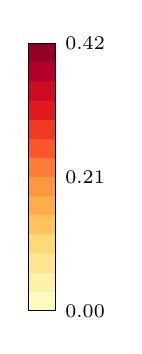
\begin{tikzpicture}
\fill[tabglobaljointnorm14] (0,0.0000) rectangle (0.35,0.2429);
\fill[tabglobaljointnorm15] (0,0.2429) rectangle (0.35,0.4857);
\fill[tabglobaljointnorm16] (0,0.4857) rectangle (0.35,0.7286);
\fill[tabglobaljointnorm17] (0,0.7286) rectangle (0.35,0.9714);
\fill[tabglobaljointnorm18] (0,0.9714) rectangle (0.35,1.2143);
\fill[tabglobaljointnorm19] (0,1.2143) rectangle (0.35,1.4571);
\fill[tabglobaljointnorm20] (0,1.4571) rectangle (0.35,1.7000);
\fill[tabglobaljointnorm6] (0,1.7000) rectangle (0.35,1.9429);
\fill[tabglobaljointnorm21] (0,1.9429) rectangle (0.35,2.1857);
\fill[tabglobaljointnorm22] (0,2.1857) rectangle (0.35,2.4286);
\fill[tabglobaljointnorm23] (0,2.4286) rectangle (0.35,2.6714);
\fill[tabglobaljointnorm24] (0,2.6714) rectangle (0.35,2.9143);
\fill[tabglobaljointnorm25] (0,2.9143) rectangle (0.35,3.1571);
\fill[tabglobaljointnorm26] (0,3.1571) rectangle (0.35,3.4000);
\draw[black,line width=0.3pt] (0,0) rectangle (0.35,3.4000);
\node[right,font=\scriptsize,anchor=west] at (0.35,3.4000) {0.42};
\node[right,font=\scriptsize,anchor=west] at (0.35,1.7000) {0.21};
\node[right,font=\scriptsize,anchor=west] at (0.35,0) {0.00};
\end{tikzpicture}
\end{minipage}
\caption{Global Wasserstein alignment, JointSheafParams (identity init), normalised. Mean $\pm$ SE across 9 datasets (First/Last), 7 for Middle (datasets with $L=2$ contribute no middle layer). Tolokers is excluded: training was unstable for this configuration (JointSheafParams, normalised=True) and no reference profile was saved. (Pooled fold/layer SE averages 0.017 across cells; not shown per cell, see text.) Cell shading: white = 0, dark red = 0.42 (max value in this table), YlOrRd colormap, same scale as Fig.~\ref{fig: RM_Norm} etc.}
\label{tab:global_joint_norm}
\end{table}


\begin{table}[H]
\centering
\definecolor{tabglobalgeneralothernorm0}{rgb}{0.8072,0.0452,0.1316}
\definecolor{tabglobalgeneralothernorm1}{rgb}{0.7792,0.026,0.139}
\definecolor{tabglobalgeneralothernorm2}{rgb}{0.7885,0.0324,0.1366}
\definecolor{tabglobalgeneralothernorm3}{rgb}{0.6821,0.0,0.149}
\definecolor{tabglobalgeneralothernorm4}{rgb}{0.7651,0.0164,0.1427}
\definecolor{tabglobalgeneralothernorm5}{rgb}{0.502,0.0,0.149}
\definecolor{tabglobalgeneralothernorm6}{rgb}{0.6896,0.0,0.149}
\definecolor{tabglobalgeneralothernorm7}{rgb}{0.7698,0.0196,0.1415}
\definecolor{tabglobalgeneralothernorm8}{rgb}{0.8353,0.0644,0.1243}
\definecolor{tabglobalgeneralothernorm9}{rgb}{0.9248,0.1739,0.1292}
\definecolor{tabglobalgeneralothernorm10}{rgb}{0.9309,0.1867,0.1326}
\definecolor{tabglobalgeneralothernorm11}{rgb}{0.9899,0.4096,0.1943}
\definecolor{tabglobalgeneralothernorm12}{rgb}{0.9948,0.6508,0.2776}
\definecolor{tabglobalgeneralothernorm13}{rgb}{0.995,0.6599,0.2816}
\definecolor{tabglobalgeneralothernorm14}{rgb}{0.9896,0.394,0.1899}
\definecolor{tabglobalgeneralothernorm15}{rgb}{0.9949,0.6554,0.2796}
\definecolor{tabglobalgeneralothernorm16}{rgb}{0.9947,0.6463,0.2756}
\definecolor{tabglobalgeneralothernorm17}{rgb}{1.0,0.9801,0.7513}
\definecolor{tabglobalgeneralothernorm18}{rgb}{1.0,0.9402,0.6538}
\definecolor{tabglobalgeneralothernorm19}{rgb}{0.9984,0.8971,0.5596}
\definecolor{tabglobalgeneralothernorm20}{rgb}{0.9961,0.8498,0.4615}
\definecolor{tabglobalgeneralothernorm21}{rgb}{0.9961,0.7634,0.3684}
\definecolor{tabglobalgeneralothernorm22}{rgb}{0.9955,0.6781,0.2894}
\definecolor{tabglobalgeneralothernorm23}{rgb}{0.9933,0.5962,0.254}
\definecolor{tabglobalgeneralothernorm24}{rgb}{0.991,0.4793,0.2143}
\definecolor{tabglobalgeneralothernorm25}{rgb}{0.9888,0.3398,0.1744}
\definecolor{tabglobalgeneralothernorm26}{rgb}{0.9463,0.2187,0.1412}
\definecolor{tabglobalgeneralothernorm27}{rgb}{0.8867,0.0996,0.1107}
\definecolor{tabglobalgeneralothernorm28}{rgb}{0.8025,0.042,0.1329}
\definecolor{tabglobalgeneralothernorm29}{rgb}{0.7046,0.0,0.149}
\definecolor{tabglobalgeneralothernorm30}{rgb}{0.5695,0.0,0.149}
\begin{minipage}{0.78\textwidth}
\centering
\renewcommand{\arraystretch}{1.2}
\begin{tabular}{lccc}
\toprule
Checkpoint & First & Middle & Last \\
\midrule
0 & \cellcolor{tabglobalgeneralothernorm0}\textcolor{white}{$0.408 \pm 0.047$} & \cellcolor{tabglobalgeneralothernorm1}\textcolor{white}{$0.419 \pm 0.062$} & \cellcolor{tabglobalgeneralothernorm1}\textcolor{white}{$0.420 \pm 0.052$} \\
1 & \cellcolor{tabglobalgeneralothernorm2}\textcolor{white}{$0.416 \pm 0.051$} & \cellcolor{tabglobalgeneralothernorm3}\textcolor{white}{$0.452 \pm 0.066$} & \cellcolor{tabglobalgeneralothernorm4}\textcolor{white}{$0.425 \pm 0.057$} \\
5 & \cellcolor{tabglobalgeneralothernorm3}\textcolor{white}{$0.450 \pm 0.050$} & \cellcolor{tabglobalgeneralothernorm5}\textcolor{white}{$0.499 \pm 0.068$} & \cellcolor{tabglobalgeneralothernorm6}\textcolor{white}{$0.448 \pm 0.063$} \\
15 & \cellcolor{tabglobalgeneralothernorm7}\textcolor{white}{$0.424 \pm 0.053$} & \cellcolor{tabglobalgeneralothernorm1}\textcolor{white}{$0.420 \pm 0.070$} & \cellcolor{tabglobalgeneralothernorm8}\textcolor{white}{$0.398 \pm 0.075$} \\
50 & \cellcolor{tabglobalgeneralothernorm9}\textcolor{white}{$0.352 \pm 0.060$} & \cellcolor{tabglobalgeneralothernorm10}\textcolor{white}{$0.348 \pm 0.098$} & \cellcolor{tabglobalgeneralothernorm9}\textcolor{white}{$0.351 \pm 0.073$} \\
200 & \cellcolor{tabglobalgeneralothernorm11}\textcolor{black}{$0.287 \pm 0.058$} & \cellcolor{tabglobalgeneralothernorm12}\textcolor{black}{$0.207 \pm 0.070$} & \cellcolor{tabglobalgeneralothernorm13}\textcolor{black}{$0.203 \pm 0.034$} \\
last & \cellcolor{tabglobalgeneralothernorm14}\textcolor{black}{$0.290 \pm 0.059$} & \cellcolor{tabglobalgeneralothernorm15}\textcolor{black}{$0.205 \pm 0.069$} & \cellcolor{tabglobalgeneralothernorm16}\textcolor{black}{$0.209 \pm 0.032$} \\
\bottomrule
\end{tabular}
\end{minipage}%
\hfill
\begin{minipage}{0.15\textwidth}
\centering
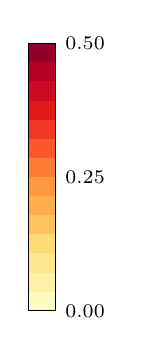
\begin{tikzpicture}
\fill[tabglobalgeneralothernorm17] (0,0.0000) rectangle (0.35,0.2429);
\fill[tabglobalgeneralothernorm18] (0,0.2429) rectangle (0.35,0.4857);
\fill[tabglobalgeneralothernorm19] (0,0.4857) rectangle (0.35,0.7286);
\fill[tabglobalgeneralothernorm20] (0,0.7286) rectangle (0.35,0.9714);
\fill[tabglobalgeneralothernorm21] (0,0.9714) rectangle (0.35,1.2143);
\fill[tabglobalgeneralothernorm22] (0,1.2143) rectangle (0.35,1.4571);
\fill[tabglobalgeneralothernorm23] (0,1.4571) rectangle (0.35,1.7000);
\fill[tabglobalgeneralothernorm24] (0,1.7000) rectangle (0.35,1.9429);
\fill[tabglobalgeneralothernorm25] (0,1.9429) rectangle (0.35,2.1857);
\fill[tabglobalgeneralothernorm26] (0,2.1857) rectangle (0.35,2.4286);
\fill[tabglobalgeneralothernorm27] (0,2.4286) rectangle (0.35,2.6714);
\fill[tabglobalgeneralothernorm28] (0,2.6714) rectangle (0.35,2.9143);
\fill[tabglobalgeneralothernorm29] (0,2.9143) rectangle (0.35,3.1571);
\fill[tabglobalgeneralothernorm30] (0,3.1571) rectangle (0.35,3.4000);
\draw[black,line width=0.3pt] (0,0) rectangle (0.35,3.4000);
\node[right,font=\scriptsize,anchor=west] at (0.35,3.4000) {0.50};
\node[right,font=\scriptsize,anchor=west] at (0.35,1.7000) {0.25};
\node[right,font=\scriptsize,anchor=west] at (0.35,0) {0.00};
\end{tikzpicture}
\end{minipage}
\caption{Global Wasserstein alignment, GeneralSheaf other Laplacian: maps trained \texttt{norm=False}, evaluated normalised. Mean $\pm$ SE across 10 datasets (First/Last), 8 for Middle (datasets with $L=2$ contribute no middle layer). (Pooled fold/layer SE averages 0.017 across cells; not shown per cell, see text.) Cell shading: white = 0, dark red = 0.50 (max value in this table), YlOrRd colormap, same scale as Fig.~\ref{fig: RM_Norm} etc.}
\label{tab:global_general_other_norm}
\end{table}


\begin{table}[H]
\centering
\footnotesize
\definecolor{tabglobalgeneralotherunnorm0}{rgb}{0.7698,0.0196,0.1415}
\definecolor{tabglobalgeneralotherunnorm1}{rgb}{0.6671,0.0,0.149}
\definecolor{tabglobalgeneralotherunnorm2}{rgb}{0.7511,0.0068,0.1464}
\definecolor{tabglobalgeneralotherunnorm3}{rgb}{0.7558,0.01,0.1452}
\definecolor{tabglobalgeneralotherunnorm4}{rgb}{0.6596,0.0,0.149}
\definecolor{tabglobalgeneralotherunnorm5}{rgb}{0.7196,0.0,0.149}
\definecolor{tabglobalgeneralotherunnorm6}{rgb}{0.7418,0.0004,0.1489}
\definecolor{tabglobalgeneralotherunnorm7}{rgb}{0.6145,0.0,0.149}
\definecolor{tabglobalgeneralotherunnorm8}{rgb}{0.7346,0.0,0.149}
\definecolor{tabglobalgeneralotherunnorm9}{rgb}{0.502,0.0,0.149}
\definecolor{tabglobalgeneralotherunnorm10}{rgb}{0.5845,0.0,0.149}
\definecolor{tabglobalgeneralotherunnorm11}{rgb}{0.7271,0.0,0.149}
\definecolor{tabglobalgeneralotherunnorm12}{rgb}{0.5545,0.0,0.149}
\definecolor{tabglobalgeneralotherunnorm13}{rgb}{0.7464,0.0036,0.1476}
\definecolor{tabglobalgeneralotherunnorm14}{rgb}{0.532,0.0,0.149}
\definecolor{tabglobalgeneralotherunnorm15}{rgb}{0.6821,0.0,0.149}
\definecolor{tabglobalgeneralotherunnorm16}{rgb}{0.6446,0.0,0.149}
\definecolor{tabglobalgeneralotherunnorm17}{rgb}{1.0,0.9801,0.7513}
\definecolor{tabglobalgeneralotherunnorm18}{rgb}{1.0,0.9402,0.6538}
\definecolor{tabglobalgeneralotherunnorm19}{rgb}{0.9984,0.8971,0.5596}
\definecolor{tabglobalgeneralotherunnorm20}{rgb}{0.9961,0.8498,0.4615}
\definecolor{tabglobalgeneralotherunnorm21}{rgb}{0.9961,0.7634,0.3684}
\definecolor{tabglobalgeneralotherunnorm22}{rgb}{0.9955,0.6781,0.2894}
\definecolor{tabglobalgeneralotherunnorm23}{rgb}{0.9933,0.5962,0.254}
\definecolor{tabglobalgeneralotherunnorm24}{rgb}{0.991,0.4793,0.2143}
\definecolor{tabglobalgeneralotherunnorm25}{rgb}{0.9888,0.3398,0.1744}
\definecolor{tabglobalgeneralotherunnorm26}{rgb}{0.9463,0.2187,0.1412}
\definecolor{tabglobalgeneralotherunnorm27}{rgb}{0.8867,0.0996,0.1107}
\definecolor{tabglobalgeneralotherunnorm28}{rgb}{0.8025,0.042,0.1329}
\definecolor{tabglobalgeneralotherunnorm29}{rgb}{0.7046,0.0,0.149}
\definecolor{tabglobalgeneralotherunnorm30}{rgb}{0.5695,0.0,0.149}
\definecolor{tabglobalgeneralotherunnorm31}{rgb}{1.0,0.9779,0.7459}
\definecolor{tabglobalgeneralotherunnorm32}{rgb}{0.9991,0.9119,0.5906}
\definecolor{tabglobalgeneralotherunnorm33}{rgb}{0.9961,0.8066,0.4149}
\definecolor{tabglobalgeneralotherunnorm34}{rgb}{1.0,0.9756,0.7405}
\definecolor{tabglobalgeneralotherunnorm35}{rgb}{0.9961,0.7922,0.3994}
\definecolor{tabglobalgeneralotherunnorm36}{rgb}{1.0,0.9291,0.6268}
\definecolor{tabglobalgeneralotherunnorm37}{rgb}{0.9961,0.7058,0.3064}
\definecolor{tabglobalgeneralotherunnorm38}{rgb}{0.9944,0.6372,0.2717}
\definecolor{tabglobalgeneralotherunnorm39}{rgb}{0.9969,0.8676,0.4976}
\definecolor{tabglobalgeneralotherunnorm40}{rgb}{0.9894,0.3785,0.1855}
\definecolor{tabglobalgeneralotherunnorm41}{rgb}{0.9248,0.1739,0.1292}
\definecolor{tabglobalgeneralotherunnorm42}{rgb}{0.9963,0.8553,0.4718}
\definecolor{tabglobalgeneralotherunnorm43}{rgb}{0.9709,0.2699,0.155}
\definecolor{tabglobalgeneralotherunnorm44}{rgb}{0.9974,0.8774,0.5183}
\definecolor{tabglobalgeneralotherunnorm45}{rgb}{0.9887,0.332,0.1722}
\definecolor{tabglobalgeneralotherunnorm46}{rgb}{0.9217,0.1675,0.1275}
\definecolor{tabglobalgeneralotherunnorm47}{rgb}{0.577,0.0,0.149}
\begin{minipage}{0.34\textwidth}
\centering
\footnotesize vs.\ topological\\[3pt]
\renewcommand{\arraystretch}{1.2}
\begin{tabular}{lccc}
\toprule
Checkpoint & First & Middle & Last \\
\midrule
0 & \cellcolor{tabglobalgeneralotherunnorm0}\textcolor{white}{$0.437 \pm 0.041$} & \cellcolor{tabglobalgeneralotherunnorm1}\textcolor{white}{$0.468 \pm 0.049$} & \cellcolor{tabglobalgeneralotherunnorm2}\textcolor{white}{$0.446 \pm 0.042$} \\
1 & \cellcolor{tabglobalgeneralotherunnorm3}\textcolor{white}{$0.443 \pm 0.039$} & \cellcolor{tabglobalgeneralotherunnorm4}\textcolor{white}{$0.472 \pm 0.048$} & \cellcolor{tabglobalgeneralotherunnorm5}\textcolor{white}{$0.455 \pm 0.039$} \\
5 & \cellcolor{tabglobalgeneralotherunnorm6}\textcolor{white}{$0.449 \pm 0.037$} & \cellcolor{tabglobalgeneralotherunnorm7}\textcolor{white}{$0.483 \pm 0.043$} & \cellcolor{tabglobalgeneralotherunnorm1}\textcolor{white}{$0.469 \pm 0.034$} \\
15 & \cellcolor{tabglobalgeneralotherunnorm8}\textcolor{white}{$0.451 \pm 0.038$} & \cellcolor{tabglobalgeneralotherunnorm9}\textcolor{white}{$0.515 \pm 0.043$} & \cellcolor{tabglobalgeneralotherunnorm10}\textcolor{white}{$0.491 \pm 0.038$} \\
50 & \cellcolor{tabglobalgeneralotherunnorm11}\textcolor{white}{$0.452 \pm 0.038$} & \cellcolor{tabglobalgeneralotherunnorm12}\textcolor{white}{$0.500 \pm 0.042$} & \cellcolor{tabglobalgeneralotherunnorm1}\textcolor{white}{$0.470 \pm 0.040$} \\
200 & \cellcolor{tabglobalgeneralotherunnorm13}\textcolor{white}{$0.447 \pm 0.034$} & \cellcolor{tabglobalgeneralotherunnorm14}\textcolor{white}{$0.506 \pm 0.042$} & \cellcolor{tabglobalgeneralotherunnorm15}\textcolor{white}{$0.466 \pm 0.042$} \\
last & \cellcolor{tabglobalgeneralotherunnorm8}\textcolor{white}{$0.451 \pm 0.035$} & \cellcolor{tabglobalgeneralotherunnorm14}\textcolor{white}{$0.505 \pm 0.042$} & \cellcolor{tabglobalgeneralotherunnorm16}\textcolor{white}{$0.476 \pm 0.043$} \\
\bottomrule
\end{tabular}
\end{minipage}%
\hfill
\begin{minipage}{0.085\textwidth}
\centering
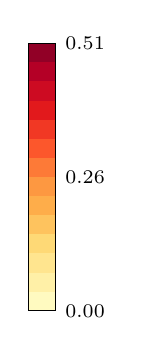
\begin{tikzpicture}
\fill[tabglobalgeneralotherunnorm17] (0,0.0000) rectangle (0.35,0.2429);
\fill[tabglobalgeneralotherunnorm18] (0,0.2429) rectangle (0.35,0.4857);
\fill[tabglobalgeneralotherunnorm19] (0,0.4857) rectangle (0.35,0.7286);
\fill[tabglobalgeneralotherunnorm20] (0,0.7286) rectangle (0.35,0.9714);
\fill[tabglobalgeneralotherunnorm21] (0,0.9714) rectangle (0.35,1.2143);
\fill[tabglobalgeneralotherunnorm22] (0,1.2143) rectangle (0.35,1.4571);
\fill[tabglobalgeneralotherunnorm23] (0,1.4571) rectangle (0.35,1.7000);
\fill[tabglobalgeneralotherunnorm24] (0,1.7000) rectangle (0.35,1.9429);
\fill[tabglobalgeneralotherunnorm25] (0,1.9429) rectangle (0.35,2.1857);
\fill[tabglobalgeneralotherunnorm26] (0,2.1857) rectangle (0.35,2.4286);
\fill[tabglobalgeneralotherunnorm27] (0,2.4286) rectangle (0.35,2.6714);
\fill[tabglobalgeneralotherunnorm28] (0,2.6714) rectangle (0.35,2.9143);
\fill[tabglobalgeneralotherunnorm29] (0,2.9143) rectangle (0.35,3.1571);
\fill[tabglobalgeneralotherunnorm30] (0,3.1571) rectangle (0.35,3.4000);
\draw[black,line width=0.3pt] (0,0) rectangle (0.35,3.4000);
\node[right,font=\scriptsize,anchor=west] at (0.35,3.4000) {0.51};
\node[right,font=\scriptsize,anchor=west] at (0.35,1.7000) {0.26};
\node[right,font=\scriptsize,anchor=west] at (0.35,0) {0.00};
\end{tikzpicture}
\end{minipage}%
\hfill
\begin{minipage}{0.34\textwidth}
\centering
\footnotesize vs.\ zero\\[3pt]
\renewcommand{\arraystretch}{1.2}
\begin{tabular}{lccc}
\toprule
Checkpoint & First & Middle & Last \\
\midrule
0 & \cellcolor{tabglobalgeneralotherunnorm31}\textcolor{black}{$0.172 \pm 0.143$} & \cellcolor{tabglobalgeneralotherunnorm32}\textcolor{black}{$0.650 \pm 0.597$} & \cellcolor{tabglobalgeneralotherunnorm33}\textcolor{black}{$1.203 \pm 1.128$} \\
1 & \cellcolor{tabglobalgeneralotherunnorm34}\textcolor{black}{$0.188 \pm 0.145$} & \cellcolor{tabglobalgeneralotherunnorm19}\textcolor{black}{$0.735 \pm 0.648$} & \cellcolor{tabglobalgeneralotherunnorm35}\textcolor{black}{$1.249 \pm 1.128$} \\
5 & \cellcolor{tabglobalgeneralotherunnorm36}\textcolor{black}{$0.530 \pm 0.331$} & \cellcolor{tabglobalgeneralotherunnorm37}\textcolor{black}{$1.537 \pm 0.908$} & \cellcolor{tabglobalgeneralotherunnorm38}\textcolor{black}{$1.785 \pm 1.072$} \\
15 & \cellcolor{tabglobalgeneralotherunnorm39}\textcolor{black}{$0.933 \pm 0.540$} & \cellcolor{tabglobalgeneralotherunnorm40}\textcolor{black}{$2.458 \pm 1.259$} & \cellcolor{tabglobalgeneralotherunnorm41}\textcolor{white}{$2.943 \pm 1.615$} \\
50 & \cellcolor{tabglobalgeneralotherunnorm42}\textcolor{black}{$1.027 \pm 0.658$} & \cellcolor{tabglobalgeneralotherunnorm43}\textcolor{white}{$2.697 \pm 1.388$} & \cellcolor{tabglobalgeneralotherunnorm7}\textcolor{white}{$3.922 \pm 1.849$} \\
200 & \cellcolor{tabglobalgeneralotherunnorm44}\textcolor{black}{$0.875 \pm 0.672$} & \cellcolor{tabglobalgeneralotherunnorm45}\textcolor{white}{$2.548 \pm 1.593$} & \cellcolor{tabglobalgeneralotherunnorm9}\textcolor{white}{$4.179 \pm 2.132$} \\
last & \cellcolor{tabglobalgeneralotherunnorm39}\textcolor{black}{$0.938 \pm 0.705$} & \cellcolor{tabglobalgeneralotherunnorm46}\textcolor{white}{$2.968 \pm 1.895$} & \cellcolor{tabglobalgeneralotherunnorm47}\textcolor{white}{$4.006 \pm 1.898$} \\
\bottomrule
\end{tabular}
\end{minipage}%
\hfill
\begin{minipage}{0.085\textwidth}
\centering
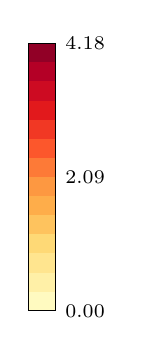
\begin{tikzpicture}
\fill[tabglobalgeneralotherunnorm17] (0,0.0000) rectangle (0.35,0.2429);
\fill[tabglobalgeneralotherunnorm18] (0,0.2429) rectangle (0.35,0.4857);
\fill[tabglobalgeneralotherunnorm19] (0,0.4857) rectangle (0.35,0.7286);
\fill[tabglobalgeneralotherunnorm20] (0,0.7286) rectangle (0.35,0.9714);
\fill[tabglobalgeneralotherunnorm21] (0,0.9714) rectangle (0.35,1.2143);
\fill[tabglobalgeneralotherunnorm22] (0,1.2143) rectangle (0.35,1.4571);
\fill[tabglobalgeneralotherunnorm23] (0,1.4571) rectangle (0.35,1.7000);
\fill[tabglobalgeneralotherunnorm24] (0,1.7000) rectangle (0.35,1.9429);
\fill[tabglobalgeneralotherunnorm25] (0,1.9429) rectangle (0.35,2.1857);
\fill[tabglobalgeneralotherunnorm26] (0,2.1857) rectangle (0.35,2.4286);
\fill[tabglobalgeneralotherunnorm27] (0,2.4286) rectangle (0.35,2.6714);
\fill[tabglobalgeneralotherunnorm28] (0,2.6714) rectangle (0.35,2.9143);
\fill[tabglobalgeneralotherunnorm29] (0,2.9143) rectangle (0.35,3.1571);
\fill[tabglobalgeneralotherunnorm30] (0,3.1571) rectangle (0.35,3.4000);
\draw[black,line width=0.3pt] (0,0) rectangle (0.35,3.4000);
\node[right,font=\scriptsize,anchor=west] at (0.35,3.4000) {4.18};
\node[right,font=\scriptsize,anchor=west] at (0.35,1.7000) {2.09};
\node[right,font=\scriptsize,anchor=west] at (0.35,0) {0.00};
\end{tikzpicture}
\end{minipage}
\caption{Global Wasserstein alignment, GeneralSheaf other Laplacian: maps trained \texttt{norm=True}, evaluated unnormalised. Mean $\pm$ SE across 10 datasets (First/Last), 8 for Middle (datasets with $L=2$ contribute no middle layer). Cell shading (each block independently scaled): white = 0, dark red = block maximum, YlOrRd colormap.}
\label{tab:global_general_other_unnorm}
\end{table}


\begin{table}[H]
\centering
\definecolor{tabglobalcrossa0}{rgb}{0.9961,0.7634,0.3684}
\definecolor{tabglobalcrossa1}{rgb}{0.9961,0.7202,0.3219}
\definecolor{tabglobalcrossa2}{rgb}{0.9888,0.3398,0.1744}
\definecolor{tabglobalcrossa3}{rgb}{0.9941,0.6235,0.2658}
\definecolor{tabglobalcrossa4}{rgb}{0.99,0.4173,0.1965}
\definecolor{tabglobalcrossa5}{rgb}{0.8493,0.074,0.1206}
\definecolor{tabglobalcrossa6}{rgb}{0.9915,0.5103,0.2231}
\definecolor{tabglobalcrossa7}{rgb}{0.8072,0.0452,0.1316}
\definecolor{tabglobalcrossa8}{rgb}{0.8773,0.0932,0.1132}
\definecolor{tabglobalcrossa9}{rgb}{0.9094,0.1419,0.1206}
\definecolor{tabglobalcrossa10}{rgb}{0.8306,0.0612,0.1255}
\definecolor{tabglobalcrossa11}{rgb}{0.5845,0.0,0.149}
\definecolor{tabglobalcrossa12}{rgb}{0.9894,0.3785,0.1855}
\definecolor{tabglobalcrossa13}{rgb}{0.7651,0.0164,0.1427}
\definecolor{tabglobalcrossa14}{rgb}{0.502,0.0,0.149}
\definecolor{tabglobalcrossa15}{rgb}{0.891,0.1036,0.1102}
\definecolor{tabglobalcrossa16}{rgb}{0.6971,0.0,0.149}
\definecolor{tabglobalcrossa17}{rgb}{0.8586,0.0804,0.1181}
\definecolor{tabglobalcrossa18}{rgb}{0.8727,0.09,0.1144}
\definecolor{tabglobalcrossa19}{rgb}{0.7838,0.0292,0.1378}
\definecolor{tabglobalcrossa20}{rgb}{1.0,0.9801,0.7513}
\definecolor{tabglobalcrossa21}{rgb}{1.0,0.9402,0.6538}
\definecolor{tabglobalcrossa22}{rgb}{0.9984,0.8971,0.5596}
\definecolor{tabglobalcrossa23}{rgb}{0.9961,0.8498,0.4615}
\definecolor{tabglobalcrossa24}{rgb}{0.9955,0.6781,0.2894}
\definecolor{tabglobalcrossa25}{rgb}{0.9933,0.5962,0.254}
\definecolor{tabglobalcrossa26}{rgb}{0.991,0.4793,0.2143}
\definecolor{tabglobalcrossa27}{rgb}{0.9463,0.2187,0.1412}
\definecolor{tabglobalcrossa28}{rgb}{0.8867,0.0996,0.1107}
\definecolor{tabglobalcrossa29}{rgb}{0.8025,0.042,0.1329}
\definecolor{tabglobalcrossa30}{rgb}{0.7046,0.0,0.149}
\definecolor{tabglobalcrossa31}{rgb}{0.5695,0.0,0.149}
\begin{minipage}{0.78\textwidth}
\centering
\renewcommand{\arraystretch}{1.2}
\begin{tabular}{lccc}
\toprule
Checkpoint & First & Middle & Last \\
\midrule
0 & \cellcolor{tabglobalcrossa0}\textcolor{black}{$0.086 \pm 0.029$} & \cellcolor{tabglobalcrossa1}\textcolor{black}{$0.096 \pm 0.014$} & \cellcolor{tabglobalcrossa2}\textcolor{white}{$0.162 \pm 0.037$} \\
1 & \cellcolor{tabglobalcrossa3}\textcolor{black}{$0.118 \pm 0.025$} & \cellcolor{tabglobalcrossa4}\textcolor{black}{$0.152 \pm 0.028$} & \cellcolor{tabglobalcrossa5}\textcolor{white}{$0.209 \pm 0.052$} \\
5 & \cellcolor{tabglobalcrossa6}\textcolor{black}{$0.139 \pm 0.027$} & \cellcolor{tabglobalcrossa7}\textcolor{white}{$0.219 \pm 0.060$} & \cellcolor{tabglobalcrossa8}\textcolor{white}{$0.203 \pm 0.050$} \\
15 & \cellcolor{tabglobalcrossa9}\textcolor{white}{$0.195 \pm 0.027$} & \cellcolor{tabglobalcrossa10}\textcolor{white}{$0.214 \pm 0.030$} & \cellcolor{tabglobalcrossa11}\textcolor{white}{$0.255 \pm 0.038$} \\
50 & \cellcolor{tabglobalcrossa12}\textcolor{black}{$0.158 \pm 0.023$} & \cellcolor{tabglobalcrossa13}\textcolor{white}{$0.228 \pm 0.046$} & \cellcolor{tabglobalcrossa14}\textcolor{white}{$0.268 \pm 0.047$} \\
200 & \cellcolor{tabglobalcrossa15}\textcolor{white}{$0.200 \pm 0.028$} & \cellcolor{tabglobalcrossa16}\textcolor{white}{$0.240 \pm 0.038$} & \cellcolor{tabglobalcrossa17}\textcolor{white}{$0.208 \pm 0.035$} \\
last & \cellcolor{tabglobalcrossa18}\textcolor{white}{$0.204 \pm 0.028$} & \cellcolor{tabglobalcrossa16}\textcolor{white}{$0.240 \pm 0.038$} & \cellcolor{tabglobalcrossa19}\textcolor{white}{$0.224 \pm 0.043$} \\
\bottomrule
\end{tabular}
\end{minipage}%
\hfill
\begin{minipage}{0.15\textwidth}
\centering
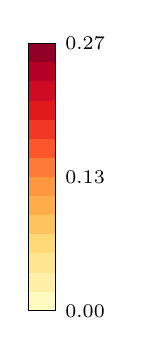
\begin{tikzpicture}
\fill[tabglobalcrossa20] (0,0.0000) rectangle (0.35,0.2429);
\fill[tabglobalcrossa21] (0,0.2429) rectangle (0.35,0.4857);
\fill[tabglobalcrossa22] (0,0.4857) rectangle (0.35,0.7286);
\fill[tabglobalcrossa23] (0,0.7286) rectangle (0.35,0.9714);
\fill[tabglobalcrossa0] (0,0.9714) rectangle (0.35,1.2143);
\fill[tabglobalcrossa24] (0,1.2143) rectangle (0.35,1.4571);
\fill[tabglobalcrossa25] (0,1.4571) rectangle (0.35,1.7000);
\fill[tabglobalcrossa26] (0,1.7000) rectangle (0.35,1.9429);
\fill[tabglobalcrossa2] (0,1.9429) rectangle (0.35,2.1857);
\fill[tabglobalcrossa27] (0,2.1857) rectangle (0.35,2.4286);
\fill[tabglobalcrossa28] (0,2.4286) rectangle (0.35,2.6714);
\fill[tabglobalcrossa29] (0,2.6714) rectangle (0.35,2.9143);
\fill[tabglobalcrossa30] (0,2.9143) rectangle (0.35,3.1571);
\fill[tabglobalcrossa31] (0,3.1571) rectangle (0.35,3.4000);
\draw[black,line width=0.3pt] (0,0) rectangle (0.35,3.4000);
\node[right,font=\scriptsize,anchor=west] at (0.35,3.4000) {0.27};
\node[right,font=\scriptsize,anchor=west] at (0.35,1.7000) {0.13};
\node[right,font=\scriptsize,anchor=west] at (0.35,0) {0.00};
\end{tikzpicture}
\end{minipage}
\caption{Global cross-comparison, Direction A (both normalised, different training objective). Mean $\pm$ SE across 10 datasets (First/Last), 8 for Middle (datasets with $L=2$ contribute no middle layer). (Pooled fold/layer SE averages 0.011 across cells; not shown per cell, see text.) Cell shading: white = 0, dark red = 0.27 (max value in this table), YlOrRd colormap, same scale as Fig.~\ref{fig: RM_Norm} etc.}
\label{tab:global_cross_a}
\end{table}


\begin{table}[H]
\centering
\definecolor{tabglobalcrossb0}{rgb}{0.9961,0.725,0.3271}
\definecolor{tabglobalcrossb1}{rgb}{0.995,0.6599,0.2816}
\definecolor{tabglobalcrossb2}{rgb}{0.99,0.4173,0.1965}
\definecolor{tabglobalcrossb3}{rgb}{0.9915,0.5103,0.2231}
\definecolor{tabglobalcrossb4}{rgb}{0.9885,0.3243,0.17}
\definecolor{tabglobalcrossb5}{rgb}{0.891,0.1036,0.1102}
\definecolor{tabglobalcrossb6}{rgb}{0.9617,0.2507,0.1499}
\definecolor{tabglobalcrossb7}{rgb}{0.6821,0.0,0.149}
\definecolor{tabglobalcrossb8}{rgb}{0.502,0.0,0.149}
\definecolor{tabglobalcrossb9}{rgb}{0.854,0.0772,0.1193}
\definecolor{tabglobalcrossb10}{rgb}{0.5845,0.0,0.149}
\definecolor{tabglobalcrossb11}{rgb}{0.547,0.0,0.149}
\definecolor{tabglobalcrossb12}{rgb}{0.8773,0.0932,0.1132}
\definecolor{tabglobalcrossb13}{rgb}{0.8446,0.0708,0.1218}
\definecolor{tabglobalcrossb14}{rgb}{0.7511,0.0068,0.1464}
\definecolor{tabglobalcrossb15}{rgb}{0.8586,0.0804,0.1181}
\definecolor{tabglobalcrossb16}{rgb}{0.9217,0.1675,0.1275}
\definecolor{tabglobalcrossb17}{rgb}{0.607,0.0,0.149}
\definecolor{tabglobalcrossb18}{rgb}{0.9371,0.1995,0.1361}
\definecolor{tabglobalcrossb19}{rgb}{1.0,0.9801,0.7513}
\definecolor{tabglobalcrossb20}{rgb}{1.0,0.9402,0.6538}
\definecolor{tabglobalcrossb21}{rgb}{0.9984,0.8971,0.5596}
\definecolor{tabglobalcrossb22}{rgb}{0.9961,0.8498,0.4615}
\definecolor{tabglobalcrossb23}{rgb}{0.9961,0.7634,0.3684}
\definecolor{tabglobalcrossb24}{rgb}{0.9955,0.6781,0.2894}
\definecolor{tabglobalcrossb25}{rgb}{0.9933,0.5962,0.254}
\definecolor{tabglobalcrossb26}{rgb}{0.991,0.4793,0.2143}
\definecolor{tabglobalcrossb27}{rgb}{0.9888,0.3398,0.1744}
\definecolor{tabglobalcrossb28}{rgb}{0.9463,0.2187,0.1412}
\definecolor{tabglobalcrossb29}{rgb}{0.8867,0.0996,0.1107}
\definecolor{tabglobalcrossb30}{rgb}{0.8025,0.042,0.1329}
\definecolor{tabglobalcrossb31}{rgb}{0.7046,0.0,0.149}
\definecolor{tabglobalcrossb32}{rgb}{0.5695,0.0,0.149}
\begin{minipage}{0.78\textwidth}
\centering
\renewcommand{\arraystretch}{1.2}
\begin{tabular}{lccc}
\toprule
Checkpoint & First & Middle & Last \\
\midrule
0 & \cellcolor{tabglobalcrossb0}\textcolor{black}{$0.082 \pm 0.030$} & \cellcolor{tabglobalcrossb1}\textcolor{black}{$0.095 \pm 0.015$} & \cellcolor{tabglobalcrossb2}\textcolor{black}{$0.132 \pm 0.025$} \\
1 & \cellcolor{tabglobalcrossb3}\textcolor{black}{$0.121 \pm 0.026$} & \cellcolor{tabglobalcrossb4}\textcolor{white}{$0.143 \pm 0.035$} & \cellcolor{tabglobalcrossb5}\textcolor{white}{$0.174 \pm 0.033$} \\
5 & \cellcolor{tabglobalcrossb6}\textcolor{white}{$0.153 \pm 0.033$} & \cellcolor{tabglobalcrossb7}\textcolor{white}{$0.210 \pm 0.055$} & \cellcolor{tabglobalcrossb8}\textcolor{white}{$0.232 \pm 0.051$} \\
15 & \cellcolor{tabglobalcrossb9}\textcolor{white}{$0.181 \pm 0.038$} & \cellcolor{tabglobalcrossb10}\textcolor{white}{$0.222 \pm 0.036$} & \cellcolor{tabglobalcrossb11}\textcolor{white}{$0.227 \pm 0.021$} \\
50 & \cellcolor{tabglobalcrossb12}\textcolor{white}{$0.176 \pm 0.027$} & \cellcolor{tabglobalcrossb13}\textcolor{white}{$0.183 \pm 0.022$} & \cellcolor{tabglobalcrossb14}\textcolor{white}{$0.201 \pm 0.017$} \\
200 & \cellcolor{tabglobalcrossb15}\textcolor{white}{$0.180 \pm 0.030$} & \cellcolor{tabglobalcrossb16}\textcolor{white}{$0.165 \pm 0.014$} & \cellcolor{tabglobalcrossb17}\textcolor{white}{$0.220 \pm 0.029$} \\
last & \cellcolor{tabglobalcrossb5}\textcolor{white}{$0.173 \pm 0.025$} & \cellcolor{tabglobalcrossb18}\textcolor{white}{$0.160 \pm 0.012$} & \cellcolor{tabglobalcrossb8}\textcolor{white}{$0.232 \pm 0.037$} \\
\bottomrule
\end{tabular}
\end{minipage}%
\hfill
\begin{minipage}{0.15\textwidth}
\centering
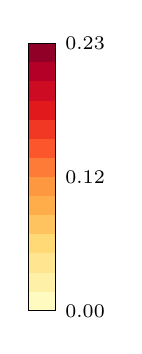
\begin{tikzpicture}
\fill[tabglobalcrossb19] (0,0.0000) rectangle (0.35,0.2429);
\fill[tabglobalcrossb20] (0,0.2429) rectangle (0.35,0.4857);
\fill[tabglobalcrossb21] (0,0.4857) rectangle (0.35,0.7286);
\fill[tabglobalcrossb22] (0,0.7286) rectangle (0.35,0.9714);
\fill[tabglobalcrossb23] (0,0.9714) rectangle (0.35,1.2143);
\fill[tabglobalcrossb24] (0,1.2143) rectangle (0.35,1.4571);
\fill[tabglobalcrossb25] (0,1.4571) rectangle (0.35,1.7000);
\fill[tabglobalcrossb26] (0,1.7000) rectangle (0.35,1.9429);
\fill[tabglobalcrossb27] (0,1.9429) rectangle (0.35,2.1857);
\fill[tabglobalcrossb28] (0,2.1857) rectangle (0.35,2.4286);
\fill[tabglobalcrossb29] (0,2.4286) rectangle (0.35,2.6714);
\fill[tabglobalcrossb30] (0,2.6714) rectangle (0.35,2.9143);
\fill[tabglobalcrossb31] (0,2.9143) rectangle (0.35,3.1571);
\fill[tabglobalcrossb32] (0,3.1571) rectangle (0.35,3.4000);
\draw[black,line width=0.3pt] (0,0) rectangle (0.35,3.4000);
\node[right,font=\scriptsize,anchor=west] at (0.35,3.4000) {0.23};
\node[right,font=\scriptsize,anchor=west] at (0.35,1.7000) {0.12};
\node[right,font=\scriptsize,anchor=west] at (0.35,0) {0.00};
\end{tikzpicture}
\end{minipage}
\caption{Global cross-comparison, Direction B (both unnormalised, different training objective). Mean $\pm$ SE across 10 datasets (First/Last), 8 for Middle (datasets with $L=2$ contribute no middle layer). (Pooled fold/layer SE averages 0.010 across cells; not shown per cell, see text.) Cell shading: white = 0, dark red = 0.23 (max value in this table), YlOrRd colormap, same scale as Fig.~\ref{fig: RM_Norm} etc.}
\label{tab:global_cross_b}
\end{table}

